\documentclass{article}

% AI4PowerGrids @ NeurIPS 2026 uses the official NeurIPS 2026 LaTeX style
% and requires double-blind review. Workshop-specific requirements govern.
\usepackage[dblblindworkshop]{neurips_2026}

\usepackage[utf8]{inputenc}
\usepackage[T1]{fontenc}
\usepackage{hyperref}
\usepackage{url}
\usepackage{booktabs}
\usepackage{amsmath}
\usepackage{amsfonts}
\usepackage{amssymb}
\usepackage{graphicx}
\usepackage{microtype}
\usepackage{xcolor}
\usepackage{capt-of}
\usepackage{flafter}
\usepackage{wrapfig}


% -----------------------------------------------------------------------------
% DRAFT-ONLY HELPERS
% Delete these prompts as prose/results are filled in.
% They do not modify NeurIPS geometry, margins, or font sizes.
% -----------------------------------------------------------------------------
\newcommand{\fillin}[1]{\textcolor{red!70!black}{\textbf{[FILL: #1]}}}
\newcommand{\draftpoint}[1]{\item \textcolor{black!70}{#1}}


% Intended OpenReview track: Position and empirical-evaluation papers.
\title{Foundation Models for Fast AC-State Evaluation:\
A GridSFM-Augmented Optimal Power Shutoff Diagnostic Study}
%remove coupling optimization with. OPS diagnostic Study%
% Use the workshop's official title in the NeurIPS workshop footer.
\workshoptitle{AI Foundations for Power Grids: From Models to Deployment at Scale}

% The dblblindworkshop style replaces author information with anonymous metadata.
\author{Anonymous Authors}

\begin{document}
\maketitle

% =============================================================================
% ABSTRACT -- final target: 5--6 prose sentences
% =============================================================================
\begin{abstract}
% \fillin{Write 5--6 sentences covering: (1) OPS setting and nonlinear AC/topology
% challenge; (2) why foundation-model state evaluation is useful; (3) GridSFM on
% GOC-500; (4) fine-tuning result; (5) downstream AC-reference result; (6) RQ1
% runtime result and/or nuanced warm-start result.}
In this work, we embed the recently released GridSFM foundation model into the existing Optimal Power Shutoff problem as a testbed for foundation model transfer to a challenging topology-changing operating regime. On the GOC-500 bus grid example, we use GridSFM as a fast electrical-state predictor for externally generated line de-energization and load-service decisions and assess its behavior across wildfire-risk scenarios. We further fine-tune GridSFM using controlled variations in both training-set size and topology distribution to examine how adaptation affects predictive fidelity and downstream OPS performance. Fine-tuning improves state and physics metrics and produces closer agreement with fixed-decision AC-OPF reference solutions, while controlled warm-start experiments show only modest solver-speed benefits. Together, the observed speedups in candidate-state prediction and the evaluator-separated formulation establish a flexible framework for further studying foundation model integration in power-system decision-making.

\end{abstract}

% =============================================================================
% 1. INTRODUCTION
% =============================================================================
\section{Introduction}

\paragraph{Optimal Power Shutoff and its computational challenge}
Wildfire mitigation creates a fundamental tradeoff for power-system operators:
preventive line de-energization during Public Safety Power Shutoff (PSPS) events
can reduce ignition exposure but may also interrupt customers and reduce served
demand \cite{Huang2023ARO}. The Optimal Power Shutoff (OPS) problem formalizes
this tradeoff as a topology-control problem in which high-risk lines are
de-energized while continuous operational recourse, including generator
redispatch, is adjusted to preserve power delivery. The original OPS formulation
uses a linearized DC power-flow representation \cite{9305959}, while subsequent
work shows that higher-fidelity AC formulations can more accurately represent
network operation at substantially greater computational cost as system size and the number of
candidate topologies increase
\cite{Rhodes2023LongST}. For a fixed operating point, AC power flow requires
solving the nonlinear active- and reactive-power balance equations, traditionally
through iterative methods such as Newton--Raphson \citep{4073219}. AC optimal power flow (AC-OPF) adds an optimization over operational controls while enforcing the nonlinear AC equations and associated operating constraints, and is commonly solved using nonlinear methods such as primal--dual interior-point algorithms \citep{Wchter2006OnTI}. In OPS, this
difficulty is compounded by the combinatorial topology search: each candidate
line-status decision creates a modified network whose operating state must be
reevaluated. 

\paragraph{Surrogates and foundation-model application}
Learned power-flow and optimal-power-flow surrogates offer one route around
repeated nonlinear solves by directly predicting electrical states, including
topology-aware models developed for contingency analysis and changing network
configurations
\citep{donnot2018fastpowersecurityanalysis,nakiganda2025graphneuralnetworksfast}.
Such models, however, are commonly specialized to a particular grid, task, or
operating distribution, motivating more reusable neural solvers and grid
foundation models designed to transfer across heterogeneous systems and
conditions \citep{puech2026gencounifiedneural,yang2026gridsfm}. GridSFM, the
released model studied here, is pretrained for AC-OPF across many grids and
operating conditions and supports system-specific adaptation through fine-tuning
\citep{yang2026gridsfm}. Within wildfire-aware power-system applications,
existing learning-based approaches have instead primarily targeted wildfire-risk
estimation or the discrete line-de-energization decision
\citep{bayani2022quantifyingriskwildfireignition,Huang2025MachineLG,HUANG2027113687,chevalier2025maximalloadsheddingverification},
rather than surrogate prediction of the resulting AC operating state.
Accordingly, we use the OPS formulation of \cite{9305959} as an operational
reference and study whether a pretrained AC-OPF foundation model can provide
fast state predictions for externally generated topology and load-service
decisions. \textbf{To the best of our knowledge, this work is the first to
integrate a pretrained grid foundation model into OPS as the surrogate AC-state
predictor used to evaluate candidate topology and load-service decisions.}
% =============================================================================
% 2. FRAMEWORK
% =============================================================================
\section{GridSFM-Augmented OPS Framework}
\begin{figure}[!htbp]
    \centering
    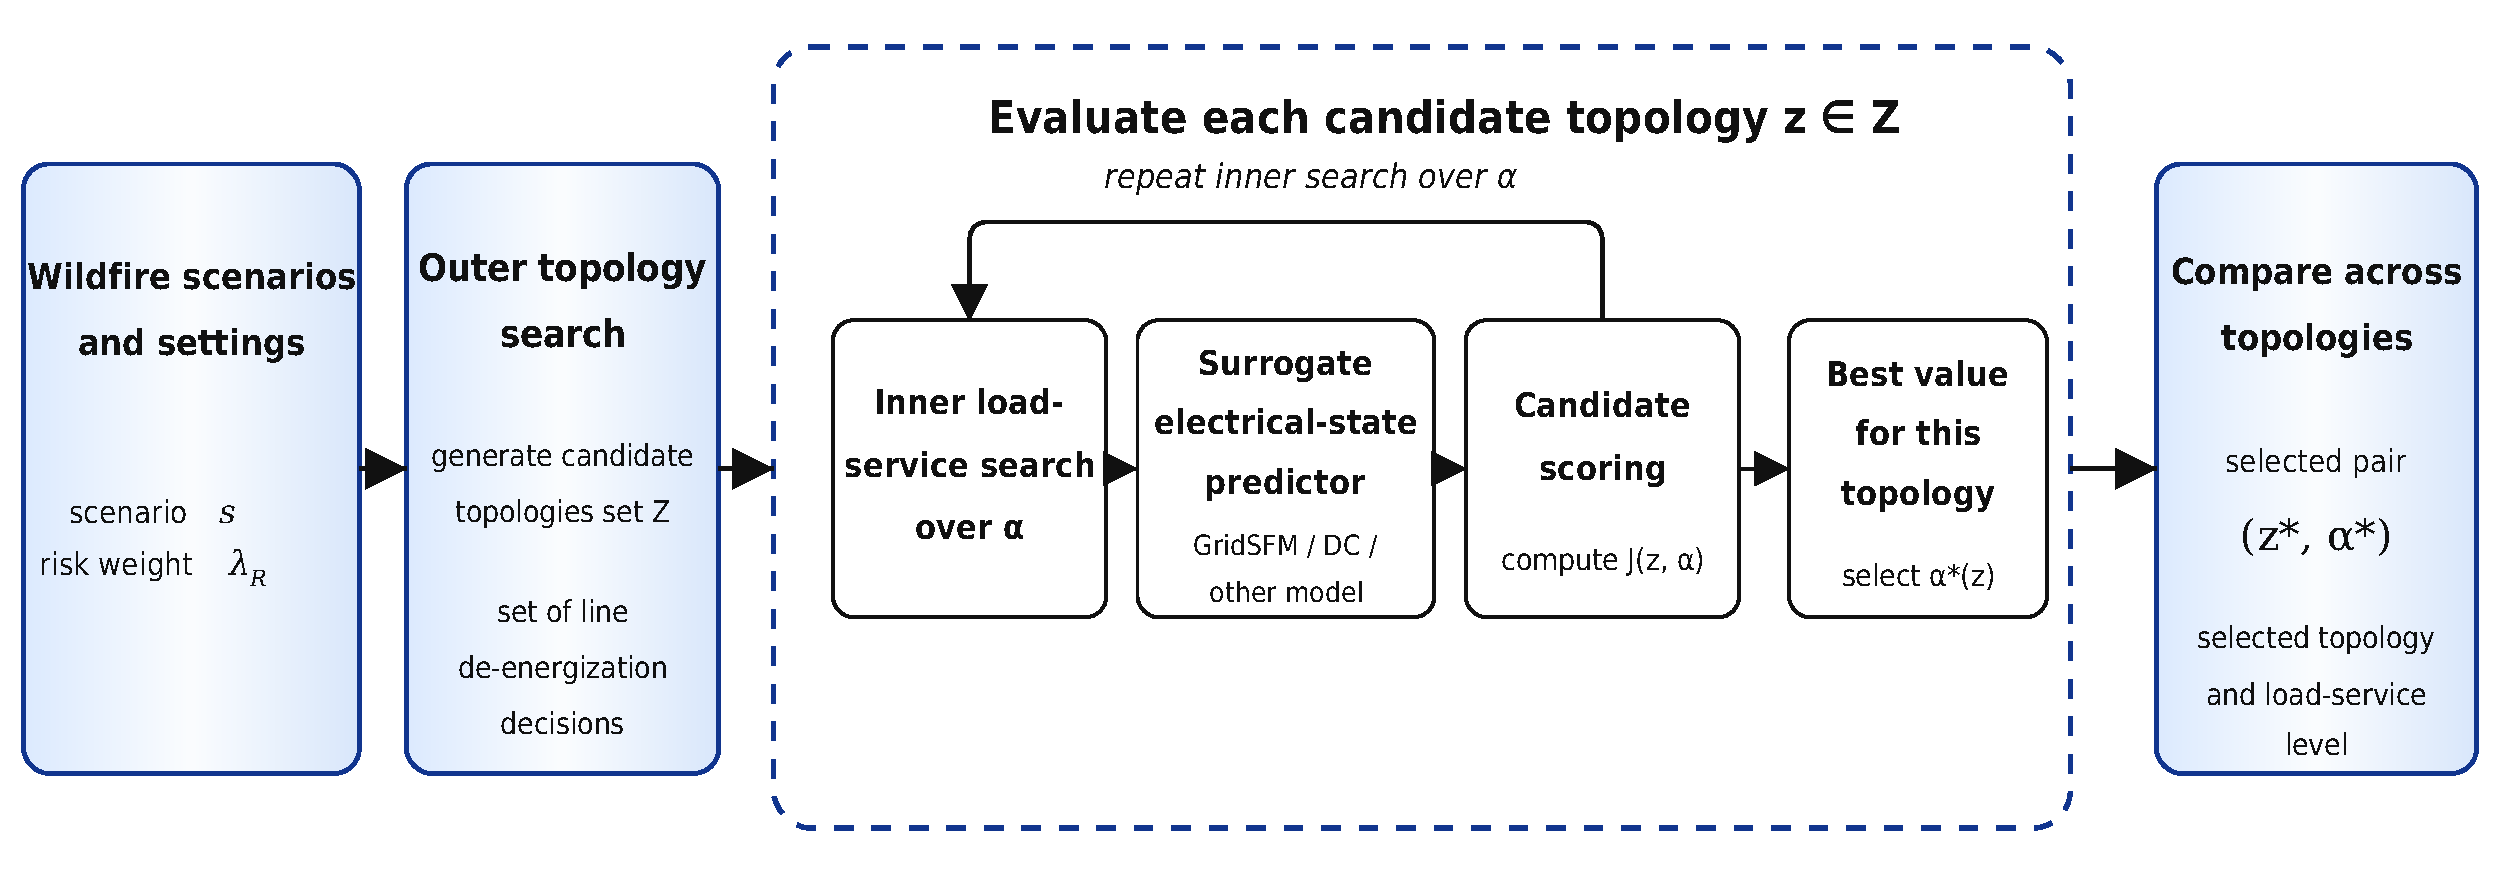
\includegraphics[width=\linewidth,
clip]{images/workflow}
    \caption{ Overview of the framework which uses the existing grid data and wildfire risk scenario to create a \textbf{fast enumeration methodology}. }
    \label{fig:pipeline}
\end{figure}
\paragraph{Outer topology search}
The outer master problem generates the set $\mathcal{Z}$ of promising
line-de-energization candidates using low-cost proxies for wildfire exposure
and load-service consequence. For a proxy risk weight $\lambda_R^M$, it solves
\begin{equation}
\begin{aligned}
\min_{z}\quad &
\lambda_R^M \widehat{R}(z)
+(1-\lambda_R^M)\widehat{L}(z) \\
\text{s.t.}\quad &
\sum_{\ell\in\mathcal{L}}(1-z_\ell)\leq K,
\qquad
z_\ell\in\{0,1\},
\qquad K=2 ,
\end{aligned}
\label{eq:topology_master}
\end{equation}
where $z_\ell=1$ and $z_\ell=0$ denote energized and de-energized lines,
respectively. The proxy terms expose their dependence on the topology decision
directly:
\begin{equation}
\widehat{R}(z)
=
\frac{\sum_{\ell\in\mathcal{L}} w_\ell z_\ell}
     {\sum_{\ell\in\mathcal{L}} w_\ell},
\qquad
\widehat{L}(z)
=
\sum_{\ell\in\mathcal{L}} c_\ell(1-z_\ell).
\label{eq:topology_proxies}
\end{equation}
Here, $w_\ell$ is a precomputed line-risk weight combining the scenario
environmental wildfire exposure with the line's baseline loading, while
$c_\ell$ is a precomputed service-impact score measuring the change in served
demand associated with removing line $\ell$ from the baseline network. 

\paragraph{GridSFM continuous recourse}
For each proposed topology $z\in\mathcal{Z}$, we optimize the load-service
vector $\alpha$ over a reduced bounded space $\mathcal{A}_B(z)$ comprising
five topology-relevant controls. Because GridSFM is treated as a
black-box electrical evaluator, we use derivative-free Powell search over this
reduced space, enabling computationally tractable evaluation across multiple candidate topologies. The best evaluated load-service decision
$\alpha^*(z)\in\arg\min_{\alpha\in\mathcal{A}_B(z)}J(z,\alpha)$ is determined
using the GridSFM-predicted AC operating state
$\hat{x}_\theta=\mathrm{GridSFM}(z,\alpha)$:
\begin{equation}
\begin{aligned}
\min_{\alpha,\hat{x}_\theta}\quad
J(z,\alpha)
&=
\lambda_R R_{\mathrm{norm}}(z,\hat{x}_\theta)
+(1-\lambda_R)L_{\mathrm{shed}}(\alpha)
+\rho_{\mathrm{phys}}P_{\mathrm{AC}}^{\mathrm{total}}(\hat{x}_\theta) \\
\text{s.t.}\quad
&\hat{x}_\theta=\mathrm{GridSFM}(z,\alpha),\\
&0\leq\alpha_i\leq1,\qquad i\in\mathcal{D},
\qquad \alpha\in\mathcal{A}_B(z).
\end{aligned}
\label{eq:gridsfm_recourse}
\end{equation}

The objective combines baseline-normalized wildfire exposure over the AC
transmission-line set $\mathcal{L}_{\mathrm{trans}}$, normalized unserved
demand over the load-bus set $\mathcal{D}$, and a decomposed physics-infeasibility
penalty:
\begin{equation}
\begin{gathered}
R_{\mathrm{norm}}(z,\hat{x}_\theta)
=
\frac{
\sum_{\ell\in\mathcal{L}_{\mathrm{trans}}}
z_\ell p_\ell^{\mathrm{env}}
\mathrm{loading}_\ell^2(z,\hat{x}_\theta)
}{
\sum_{\ell\in\mathcal{L}_{\mathrm{trans}}}
p_\ell^{\mathrm{env}}
(\mathrm{loading}_\ell^{\mathrm{base}})^2
},
\qquad
L_{\mathrm{shed}}(\alpha)
=
\frac{
\sum_{i\in\mathcal{D}}
P_{d,i}^{\mathrm{base}}(1-\alpha_i)
}{
\sum_{i\in\mathcal{D}}
P_{d,i}^{\mathrm{base}}
},
\\[2pt]
P_{\mathrm{AC}}^{\mathrm{total}}
=
P_{\mathrm{AC}}^{\mathrm{oper}}
+
P_{\mathrm{AC}}^{P/Q}
+
P_{\mathrm{AC}}^{\mathrm{model}} .
\end{gathered}
\label{eq:recourse_terms}
\end{equation}
Here, $R_{\mathrm{norm}}$ compares wildfire-weighted post-decision loading
against the intact baseline, $L_{\mathrm{shed}}$ measures the fraction of
baseline demand not served with $\alpha_i$ denoting the served fraction at
load bus $i$, and $P_{\mathrm{AC}}^{\mathrm{total}}$ aggregates operational,
active/reactive power-balance, and model-consistency constraint violations,
where Table~\ref{tab:rq1-physics} provides a representative decomposition.

After retaining $\alpha^*(z)$ for each candidate topology, the final OPS
solution is selected across the evaluated $(z,\alpha^*(z))$ pairs. Full
formulation details, search settings, term definitions, islanding treatment,
and differences from the original OPS formulation are provided in the Appendix.

% =============================================================================
% 3. RESULTS ORGANIZED BY RESEARCH QUESTION
% =============================================================================
\section{Results}
\subsection{RQ1: GridSFM prediction performance in topology-changing OPS}
\begin{figure}[!htbp]
    \centering
    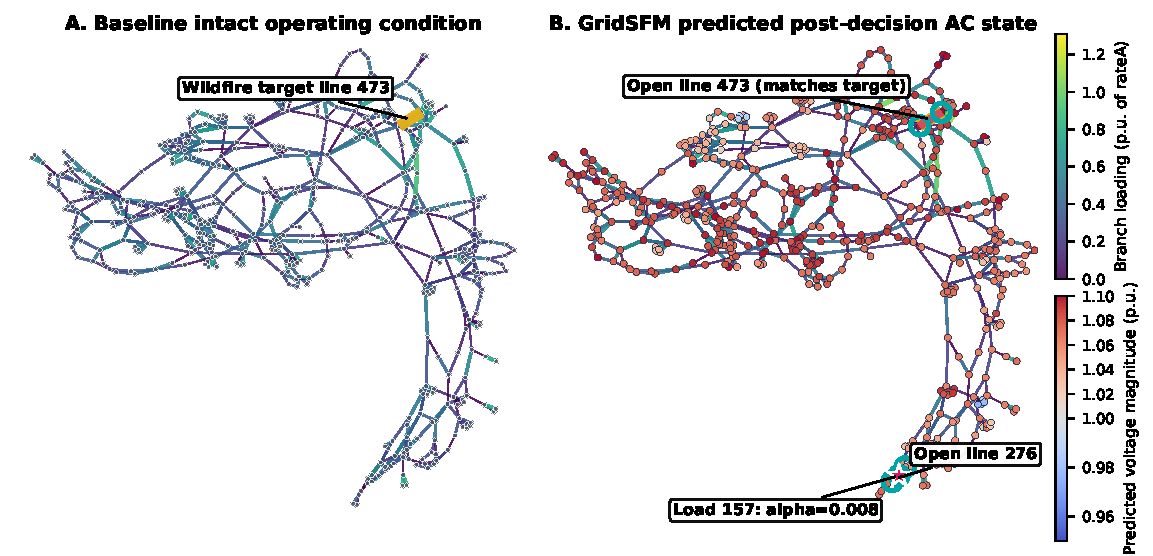
\includegraphics[
        width=\linewidth,
        height=2.45in,
        keepaspectratio
    ]{images/rq1_representative_grid_v2.pdf}
    \caption{A depiction of the OPS workflow at use through the baseline operating
    condition and final OPS decision using the J-S1 wildfire scenario at
    $\lambda_R=0.8$.}
    \label{fig:rq1-grid}
\end{figure}

\noindent\textbf{Workflow and state response}\enspace
We first evaluate GridSFM on the diagnostic J-S1 setting, which contains one
high-wildfire-risk line with relatively low expected service impact and is
designed to test whether OPS decisions follow the intended risk pattern.
At \(\lambda_R=0.8\), the solution opens the targeted high-risk branch 473 and branch 276 and reduces load 157 to \(\alpha_{\mathrm{eff}}=0.0081\). Predicted voltages remain within limits up to numerical tolerance. In this diagnostic setting, such interpretable state predictions provide a controlled
proof of concept for using GridSFM inside OPS before considering larger,
economically detailed wildfire-operation studies.


\noindent
\begin{minipage}[t]{0.49\linewidth}
\vspace{0pt}
\textbf{Physics consistency under topology shift}\enspace
Table~\ref{tab:rq1-physics} qualifies the preceding state prediction through
explicit AC-physics constraint violations modeled in the objective function.
Overall physics consistency degrades under the topology-changing operating
regime, motivating the fine-tuning study in RQ2. Model-consistency violations
remain zero across the evaluated states and serve primarily as a diagnostic
for errors in the GridSFM evaluation workflow.
\end{minipage}%
\hfill%
\begin{minipage}[t]{0.48\linewidth}
\vspace{-3pt}
\centering
\begingroup
\setlength{\abovecaptionskip}{0pt}
\setlength{\belowcaptionskip}{2pt}

\captionof{table}{Physics penalties for the J-S1 example.}
\label{tab:rq1-physics}

\footnotesize
\renewcommand{\arraystretch}{0.92}
\begin{tabular*}{\linewidth}{@{\extracolsep{\fill}}lcc@{}}
\toprule
Diagnostic & Intact & Modified \\
\midrule
Voltage-limit penalty
    & 0 & 0 \\
Thermal-limit penalty
    & $3.14{\times}10^{-6}$ & $1.58{\times}10^{-4}$ \\
Generator-bound penalty
    & 0 & 0 \\
Source-less-service penalty
    & 0 & 0 \\
$\mathbf{P_{\mathrm{AC}}^{\mathrm{oper}}}$
    & $\mathbf{3.14{\times}10^{-6}}$
    & $\mathbf{1.58{\times}10^{-4}}$ \\
Active-power balance MSE
    & 0.0768 & 0.0887 \\
Reactive-power balance MSE
    & 0.0250 & 0.0792 \\
$\mathbf{P_{\mathrm{AC}}^{P/Q}}$
    & $\mathbf{0.1018}$ & $\mathbf{0.1679}$ \\
\midrule
$\mathbf{P_{\mathrm{AC}}^{\mathrm{Total}}}$
    & $\mathbf{0.1018}$ & $\mathbf{0.1681}$ \\
\bottomrule
\end{tabular*}

\endgroup
\end{minipage}%
\par\vspace{-3pt}



\noindent\textbf{Candidate-state evaluation cost}\enspace
Across 54 unique fixed $(z,\alpha)$ instances, GridSFM achieves median
$3.35\times$ and $3.59\times$ speedups over IPOPT for the core forward pass
and complete candidate-to-state evaluation, respectively. Combined with the
increased physics residuals under topology change, these results expose a
clear speed--fidelity tradeoff: GridSFM substantially accelerates state
evaluation, but improved physical fidelity remains necessary for reliable OPS
assessment. Full timing distributions and paired confidence intervals are
reported in the Appendix.

% -------------------------------------------------------------------------
\subsection{RQ2: Does fine-tuning improve GridSFM?}

\noindent\textbf{Fine-tuning performance}\enspace
Model 1 denotes the released GridSFM checkpoint. Model 2 fine-tunes Model 1 on 1,000
GOC-500 full topology cases; Model 3 continues Model 2 with 500 additional Full Topology samples,
whereas Model 4 instead uses 500 N-1 samples. 

\begin{table}[!htbp]
    \centering
    \caption{Fine-tuning evaluation and physics transfer.}
    \label{tab:finetune}
    \scriptsize
    \renewcommand{\arraystretch}{0.90}
    \setlength{\tabcolsep}{2.0pt}
    \makebox[\linewidth][c]{%
\begin{tabular}{@{}lcccccccc@{}}
        \toprule
        &
        \multicolumn{2}{c}{FullTop test} &
        \multicolumn{2}{c}{N-1 test} &
        \multicolumn{2}{c}{$P_{\mathrm{AC}}^{\mathrm{oper}}$} &
        \multicolumn{2}{c}{$P_{\mathrm{AC}}^{P/Q}$} \\
        \cmidrule(lr){2-3}
        \cmidrule(lr){4-5}
        \cmidrule(lr){6-7}
        \cmidrule(lr){8-9}

        Model &
        Loss & Br.-P MAE &
        Loss & Br.-P MAE &
        Intact & Modified &
        Intact & Modified \\
        \midrule

        1 &
        0.09330 & 0.07451 &
        0.11847 & 0.07688 &
        $3.14{\times}10^{-6}$ & $1.58{\times}10^{-4}$ &
        0.1018 & 0.1679 \\

        2 &
        0.04079 & 0.04048 &
        0.07015 & 0.04360 &
        0 & $1.07{\times}10^{-4}$ &
        0.0131 & 0.0738 \\

        3 &
        \textbf{0.03811} & \textbf{0.03502} &
        0.06824 & 0.03869 &
        0 & $1.09{\times}10^{-4}$ &
        \textbf{0.0080} & 0.0633 \\

        4 &
        0.04038 & 0.03605 &
        \textbf{0.05680} & \textbf{0.03804} &
        0 & $1.22{\times}10^{-4}$ &
        0.0128 & \textbf{0.0312} \\

        \bottomrule
    \end{tabular}%
    }
\end{table}

Fine-tuning substantially improves both predictive performance and physics
consistency relative to the released GridSFM checkpoint
(Table~\ref{tab:finetune}). Although the topology-changing J-S1 regime still
induces a structural shift between intact and modified states, all fine-tuned
models substantially reduce the resulting AC-physics residuals. The lowest
modified-state residual is obtained after adaptation with N-1 samples,
suggesting that explicit exposure to topology variation is particularly useful
for improving GridSFM behavior under OPS-induced network changes. These results
motivate further study of topology-aware training/fine-tuning strategies for adapting
foundation models to structurally shifted operating regimes. Full prediction
metrics, residual constructions, and operational penalty definitions are
provided in the Appendix.



% -------------------------------------------------------------------------
\subsection{RQ3: Do model improvements transfer to OPS behavior?}

\noindent
\begin{minipage}[t]{0.43\linewidth}
\vspace{0pt}
\textbf{Native GridSFM tradeoffs.}\enspace
We compare Model 1--Model 4 within the common GridSFM evaluator, with all
checkpoints sharing the same AC-loading definition, physics penalty, and search
procedure. Fine-tuning shifts the empirical wildfire-risk/load-service
tradeoffs toward lower native objective values
(Figure~\ref{fig:pareto}). These fronts summarize the evaluated search budget
rather than an exhaustive AC Pareto frontier.
\end{minipage}%
\hfill%
\begin{minipage}[t]{0.54\linewidth}
\vspace{0pt}
\centering
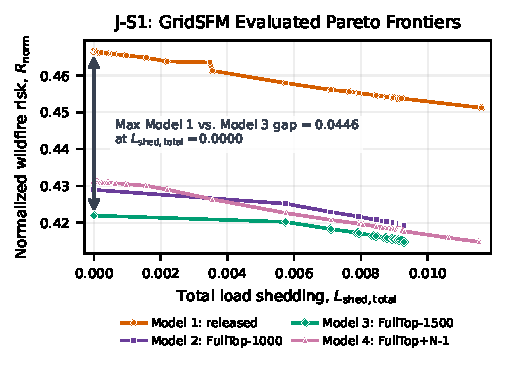
\includegraphics[
    width=\linewidth,
    keepaspectratio
]{images/gridsfm_pareto_j-s1.pdf}
\vspace{-3pt}
\captionof{figure}{GridSFM Pareto tradeoffs on J-S1.}
\label{fig:pareto}
\end{minipage}%
\par\vspace{-1pt}

\noindent\textbf{Transfer to the AC-OPF reference.}\enspace
More importantly, the gains observed during fine-tuning persist when selected
OPS decisions are reevaluated against the common fixed-decision AC-OPF
reference. From Model 1 to Model 3, state NRMSE decreases from 0.2073 to
0.1206, mean absolute wildfire-risk discrepancy from 0.0750 to 0.0176, and
mean absolute objective discrepancy from 0.0308 to 0.0051, corresponding to
approximately 42\%, 76\%, and 83\% reductions. Thus, improved standalone
GridSFM fidelity translates into substantially better downstream agreement
with the higher-fidelity AC evaluation.

\noindent\textbf{Transfer to the AC-OPF reference.}\enspace
More importantly, the gains observed during fine-tuning persist when selected
OPS decisions are reevaluated against the common fixed-decision AC-OPF
reference. From Model 1 to Model 3, state NRMSE decreases from 0.2073 to
0.1206, mean absolute wildfire-risk discrepancy decreases from 0.0750 to
0.0176, and mean absolute objective discrepancy decreases from 0.0308 to
0.0051. These correspond to approximately 42\%, 76\%, and 83\% reductions,
respectively. Thus, improved standalone GridSFM fidelity translates into
substantially better downstream agreement with the higher-fidelity AC
evaluation.

\noindent\textbf{Controlled warm starts.}\enspace
We finally test whether improved state prediction also accelerates nonlinear
AC-OPF solution. Across the 75 fixed Reference~A instances, median IPOPT
iteration counts are 33 from a cold start, 30 from DC, and 31 for each GridSFM
checkpoint. Median solve times are 5.113~s for cold initialization, 5.075~s
for DC, and 5.104, 5.039, 5.055, and 5.067~s for Model 1--Model 4,
respectively. Informed electrical states provide modest benefits over cold
initialization, but improved GridSFM prediction accuracy does not induce a
monotonic or proportional IPOPT speedup. Reference~B provides a complementary
diagnostic of whether the selected topology itself restricts AC-load
deliverability; detailed results are deferred to the Appendix.

% =========================================================================
\section{Conclusion and Outlook}

%SCOPE SHOULD CLARIFY THE LIMITATIONS WITH THE EVALUATED DECISIONS%
\paragraph{Scope and findings}
This work provides a controlled diagnostic study of integrating a pretrained
grid foundation model into topology-changing OPS as a surrogate AC-state
predictor. On GOC-500, base GridSFM produces operationally interpretable
candidate states while achieving a median $3.59\times$ speedup over
fixed-decision AC-OPF at the complete candidate-to-state boundary. The
topology-changing regime also increases physics residuals, motivating
system-specific adaptation; subsequent fine-tuning improves predictive fidelity
and substantially reduces disagreement with the fixed-decision AC-OPF
reference. These improvements, however, do not translate proportionally into
faster nonlinear-solver convergence. As the experiments use constructed
wildfire scenarios and a bounded enumeration of topology and load-service
candidates, the results establish a controlled proof of concept rather than a
deployment-ready OPS policy.

%SPECIFY WITH THE GRAY BOX FORMULATION IDEA TOWARDS THE FACT THAT THIS IS AN ENUMERATION STUDY. FURTHER WORK ON ALGORITHMS NOTABLY TO COMBINE THE TOPOLOGY DECISIONS AND CONTINUOUS RECOURSE PROCESS TOGETHER IS AN IMPORTANT FOCUS%
\paragraph{Outlook}
The evaluator-separated formulation provides a basis for extending
foundation-model-guided power-system decision making beyond this diagnostic
setting. Security-constrained OPS can test whether learned state prediction
remains useful when shutoff decisions must preserve robustness to subsequent
contingencies \citep{Rhodes2023SecurityCO}, while larger systems with realistic
wildfire-risk data and explicit economic and reliability objectives can assess
the operational value of the observed speed--fidelity tradeoff. Future work can
also compare emerging grid foundation models under a common decision framework
and move beyond external state prediction toward gray-box formulations in which
foundation-model states and derivatives are coupled directly with the
continuous optimization algorithm.
% =============================================================================
% AI / LLM DISCLOSURE -- workshop CFP says reportable use, if any, goes here.
% The NeurIPS 2026 handbook states basic editing/writing assistance need not be
% documented. If your final use becomes reportable under the policy, insert an
% unnumbered statement immediately before References.
% =============================================================================
% \section*{Generative AI / LLM disclosure}
% \fillin{Include only if required by the final NeurIPS/AI4PowerGrids policy.}

% =============================================================================
% END OF 4-PAGE MAIN CONTENT BUDGET
% Everything below is outside the AI4PowerGrids 4-page main-content limit.
% =============================================================================

% =============================================================================
% REFERENCES -- unlimited, outside the 4-page main-content limit
% =============================================================================

\bibliographystyle{plain}
\bibliography{ref}



% =============================================================================
% OPTIONAL TECHNICAL APPENDIX -- permitted; reviewers are not obligated to read it
% =============================================================================
\newpage
\appendix
%APPENDIX SHOULD INCLUDE THE FOLLOWING: TIMING RESULTS, OPS FORMULATION INCLUDING THE FULL SET OF DEFINITIONS FOR EACH TERM - HOW THE PENALTIES ARE CONSIDERED ALONGSIDE THE WEIGHTS, MORE RESULTS FROM S1-S3 AND LAMBDA SWEEPS - DIFFERENCE IN TIMINGS, THE REFERENCES, AND FINALLY THE COMPARISON WITH HEURISTICS.%
\section{Additional RQ1 Timing Results}

\begin{table}[!htbp]
    \centering
    \caption{Model 1 candidate-state evaluation timing over 54 unique fixed
    decisions. Times report median [IQR]; speedups are paired medians with
    95\% bootstrap intervals.}
    \label{tab:rq1-runtime-full}
    \small
    \begin{tabular}{lccc}
        \toprule
        Boundary & GridSFM (s) & AC-OPF ref. (s) & Speedup \\
        \midrule
        Core compute &
        0.222 [0.220--0.224] &
        0.746 [0.719--0.777] &
        3.35$\times$ [3.31--3.45] \\
        State evaluator &
        0.297 [0.293--0.305] &
        1.092 [1.012--1.116] &
        3.59$\times$ [3.48--3.68] \\
        \bottomrule
    \end{tabular}
\end{table}
\section{Full OPS formulation}
\label{app:formulation}
\begin{itemize}
    \draftpoint{Decision variables, topology budget, effective load service, and source-less island rule.}
    \draftpoint{Load-shedding definition; wildfire-risk equation and intact AC normalization; PAC physics penalty; full GridSFM candidate merit.}
    \draftpoint{Outer topology proxy and bounded $\alpha$ search.}
\end{itemize}

\section{Evaluator and AC-reference definitions}
\begin{itemize}
    \draftpoint{DC active-power loading versus GridSFM apparent-power loading and the native-objective comparability boundary.}
    \draftpoint{Reference A fixed-$(z,\alpha)$ economic AC-OPF; Reference B maximum-load-delivery problem and economic tie-break.}
    \draftpoint{Solver tolerances and interpretation of successful IPOPT solutions.}
\end{itemize}

\section{Experimental and supplementary details}
\begin{itemize}
    \draftpoint{J-S1/J-S2/J-S3 construction; $\lambda_R$ sweep; $K\leq2$; topology and continuous candidate budgets.}
    \draftpoint{Model 1--Model 4 fine-tuning splits, training settings, sealed full topology/N-1 metrics.}
    \draftpoint{RQ1 timing protocol, unique-instance provenance, full timing distributions, and paired speedup statistics.}
    \draftpoint{All scenario Pareto plots; full Reference A/B results; full warm-start paired results.}
\end{itemize}

% =============================================================================
% REQUIRED AI4POWERGRIDS DOMAIN EVALUATION CHECKLIST
% Workshop CFP explicitly says this checklist is required and the standard
% NeurIPS Paper Checklist should NOT be included.
% This section is outside the 4-page main-content limit.
% =============================================================================
\section*{AI4PowerGrids domain evaluation checklist}
\begin{enumerate}
    \item \textbf{Physics feasibility.}
    \fillin{State where full-AC feasibility / constraint-violation statistics are reported (e.g., RQ1/RQ3 and appendix), or justify N/A.}

    \item \textbf{Out-of-distribution evaluation.}
    \fillin{State where unseen topology / operating-distribution evaluation is reported; distinguish FullTop and N-1 exposure carefully.}

    \item \textbf{Failure modes.}
    \fillin{Point to worst-case/tail/qualitative physics or prediction failures, or explicitly state the available failure-mode evidence and its limits.}

    \item \textbf{System-level effect.}
    \fillin{Point to RQ3: native-to-reference OPS agreement, Pareto behavior, and controlled warm-start study.}

    \item \textbf{Data and code.}
    \fillin{Provide anonymous submission-time release plan or acceptance-time release plan; state any restrictions.}
\end{enumerate}

% IMPORTANT: Do NOT include the standard NeurIPS Paper Checklist for this workshop.

\end{document}
